\documentclass[12pt, letterpaper]{article}
\usepackage[utf8]{inputenc}
\usepackage{graphicx}
\usepackage{wrapfig}
\usepackage{caption}
\usepackage{microtype}
\usepackage{listings}
\usepackage{xcolor-solarized}
\usepackage{booktabs}

\usepackage{hyperref}

\definecolor{dkgreen}{rgb}{0,0.6,0}
\definecolor{gray}{rgb}{0.5,0.5,0.5}
\definecolor{mauv}{rgb}{0.58,0,0.82}

\lstset{frame=tb,
    language=Java,
    aboveskip=3mm,
    belowskip=3mm,
    showstringspaces=false,
    columns=flexible,
    basicstyle={\small\ttfamily},
    numbers=none,
    numberstyle=\tiny\color{gray},
    keywordstyle=\color{blue},
    commentstyle=\color{dkgreen},
    stringstyle=\color{mauve},
    breaklines=true,
    breakatwhitespace=true,
    tabsize=3
}


\newcommand\YAMLcolonstyle{\color{red}\mdseries}
\newcommand\YAMLkeystyle{\color{black}\bfseries}
\newcommand\YAMLvaluestyle{\color{blue}\mdseries}

\makeatletter

    % here is a macro expanding to the name of the language
% (handy if you decide to change it further down the road)
    \newcommand\language@yaml{yaml}

    \expandafter\expandafter\expandafter\lstdefinelanguage
    \expandafter{\language@yaml}
{
    keywords={true,false,null,y,n},
        keywordstyle=\color{darkgray}\bfseries,
        basicstyle=\YAMLkeystyle,                                 % assuming a key comes first
            sensitive=false,
        comment=[l]{\#},
        morecomment=[s]{/*}{*/},
        commentstyle=\color{purple}\ttfamily,
        stringstyle=\YAMLvaluestyle\ttfamily,
        moredelim=[l][\color{orange}]{\&},
        moredelim=[l][\color{magenta}]{*},
        moredelim=**[il][\YAMLcolonstyle{:}\YAMLvaluestyle]{:},   % switch to value style at :
            morestring=[b]',
        morestring=[b]",
        literate =    {---}{{\ProcessThreeDashes}}3
        {>}{{\textcolor{red}\textgreater}}1
    {|}{{\textcolor{red}\textbar}}1
    {\ -\ }{{\mdseries\ -\ }}3,
}

% switch to key style at EOL
\lst@AddToHook{EveryLine}{\ifx\lst@language\language@yaml\YAMLkeystyle\fi}
\makeatother

\newcommand\ProcessThreeDashes{\llap{\color{cyan}\mdseries-{-}-}}


\colorlet{punct}{red!60!black}
\definecolor{background}{HTML}{EEEEEE}
\definecolor{delim}{RGB}{20,105,176}
\colorlet{numb}{magenta!60!black}

\lstdefinelanguage{json}{
    showstringspaces=false,
    breaklines=true,
    literate=
     *{0}{{{\color{numb}0}}}{1}
      {1}{{{\color{numb}1}}}{1}
      {2}{{{\color{numb}2}}}{1}
      {3}{{{\color{numb}3}}}{1}
      {4}{{{\color{numb}4}}}{1}
      {5}{{{\color{numb}5}}}{1}
      {6}{{{\color{numb}6}}}{1}
      {7}{{{\color{numb}7}}}{1}
      {8}{{{\color{numb}8}}}{1}
      {9}{{{\color{numb}9}}}{1}
      {:}{{{\color{punct}{:}}}}{1}
      {,}{{{\color{punct}{,}}}}{1}
      {\{}{{{\color{delim}{\{}}}}{1}
      {\}}{{{\color{delim}{\}}}}}{1}
      {[}{{{\color{delim}{[}}}}{1}
      {]}{{{\color{delim}{]}}}}{1},
}

\usepackage{protobuf/lang}  % include language definition for protobuf
\usepackage{protobuf/style} % include custom style for proto declarations.

\graphicspath{ {./images/} }

\title{Lab 1: Introduction to Serialization}
\author{Neil Johari $<$\href{mailto:njohari@umich.edu}
       {njohari@umich.edu}$>$}

\date{\today}

\begin{document}

\maketitle

\section{Introduction}
\begin{wrapfigure}{L}{0.5\textwidth}
    \begin{center}
        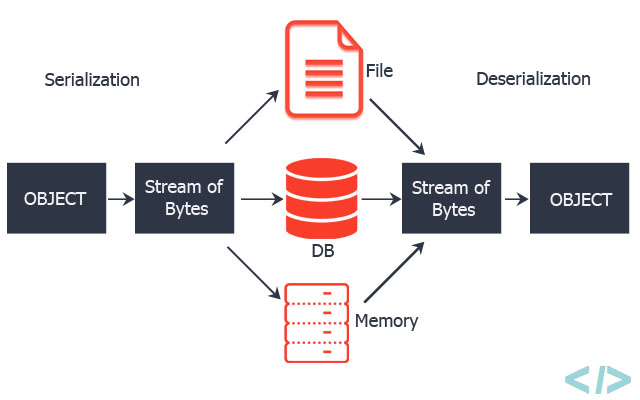
\includegraphics[width=0.5\textwidth]{header-picture}
    \end{center}
    \caption*{pc: \href{https://www.codenuclear.com/serialization-deserialization-java/}{codenuclear.com}}
\end{wrapfigure}

Serialization (also known as marshalling) is a powerful data storage technique employed to deal with data that is intended to transmit or store the state of objects in a computer program.

During serialization, data structures and objects are converted into a stream of bytes, which then can be stored on a disk or shared over a network. Serialization becomes useful when data must be reconstructed via deserialization (or unmarshalling): the serialized stream is used to recreate the original object in memory, and the new object is semantically equivalent to when it was serialized. 

In this lab we will explore a brief history of various serialization techniques and understand how computer files work. Then we will investigate how we can implement these techniques into microcontroller driven systems. In the following labs, we will actually implement two examples of serialization in ArduinoC and corresponding deserialization. 


\section{History}
In the 1990s, Extensible Markup Language (XML) was developed by the W3C as a file format intended to structure data documents such that they were both easily readable by humans and also parsable in computer programs. Please note that XML is not the same thing as HTML; HTML is used to describe how a page should be presented in browsers, while XML describes content.


Later, Javascript Object Notation (JSON) and YAML were pushed as light-weight alternatives to XML. JSON is often used to send data back and forth between web clients and servers, while YAML has become popular for configuration files. Since YAML 1.2, YAML is fully compatible with JSON as an official subset. \cite{ben-kiki_evans_net_2009}. 


\lstinputlisting[language=XML, caption=Sample XML document \cite{xml_tutorial}]{code/sample-xml.xml}
\lstinputlisting[language=yaml, caption=Sample YAML document \cite{yaml_json_comparison}]{code/sample-yaml.yaml}
\lstinputlisting[language=json, caption=Sample JSON document \cite{yaml_json_comparison}]{code/sample-yaml.yaml}


\section{Terminology and Background}
This section covers some basic IO terminology which you may find useful as you proceed through labs where you will implement serialization libraries on your own.

\subsection{Streams}
Streams are a useful abstraction for handling incoming or outgoing data (or both). A stream is an abstract series of objects which may not all be available at any given moment. A common analogy is that streams are like conveyor belts which can either deliver objects towards or away from you; you can either place objects onto the belt or take objects off it \cite{so_streams}.

A use of streams you may be familiar with is the \texttt{sed} (stream editor) utility in Unix. The utility can process files line-by-line without ever loading the entire file at once. Streams are also the abstraction used to support network sockets. 

Understanding what streams are is important as most serialization techniques yield a binary stream representing the serialized object. 


\subsection{Computer Files}
Computer files are simply data containers, nothing more. The data is often contained in a 1D byte array and. Typically, the file extension carries meaning as to how a program should read the contents of the file. Many file types also reserve a few bytes in the beginning of the file to store metadata about the file.

In terms of how the data within the file is organized, the file type has full control how data should be split into smaller units. For instance, plain text files often use newlines as a delimeter between "lines". It is important to realize that a computer file is very versatile; it is not difficult to invent a new file type, which we will do in a later lab. 


\section{Serialization in Microcontrollers}
In the next labs we will focus on importing and using two serialization frameworks on an Arduino Nano. We will pipe our stream output into a file using the OpenLog, and will later access this file on our computers and deserialize the written data. Here, we will investigate what factors must be considered when working on a microcontroller. 

\subsection{Constraints}
An Arduino Nano has 32 KB of flash memory, of which 2 KB are used by the bootloader. There are a maximum of 30720 bytes left for your program.  It's important to realize that going past $\approx 70$\% of the allocated memory will lead to a warning stating \texttt{Low memory available, stability problems may occur}. 

We will try to be careful when choosing a library so that the memory footprint is low. If you run into a warning like this, try to optimize your program! There are many resources online which give helpful tips on optimization, and you can always reach out to your IA to get more information. 

\subsection{Libraries}
\subsubsection{ArduinoJson}
\subsubsection{Nanopb}




\bibliographystyle{IEEEtran}
\bibliography{references}
\end{document}
